\documentclass[a4paper]{article}
\usepackage{INTERSPEECH2014,amssymb,amsmath,epsfig}

\usepackage[utf8]{inputenc}
\usepackage{amsmath}
\usepackage{multirow}
\usepackage{caption}
\usepackage{subcaption}
\usepackage{dblfloatfix}

\setcounter{page}{1}
\sloppy     					% better line breaks
\ninept
\def\reg{{\rm\ooalign{\hfil
     \raise.07ex\hbox{\scriptsize R}\hfil\crcr\mathhexbox20D}}}



\title{Hybrid language models for speech transcription}

\makeatletter
\def\name#1{\gdef\@name{#1\\}}
\makeatother \name{{\em Luiza Orosanu$^{1,2,3}$, Denis Jouvet$^{1,2,3}$}}

\address{Speech Group, LORIA\\
$^1$ Inria, Villers-lès-Nancy, F-54600, France \\
$^2$ Université de Lorraine, LORIA, UMR 7503, Villers-lès-Nancy, F-54600, France \\
$^3$ CNRS, LORIA, UMR 7503, Villers-lès-Nancy, F-54600, France \\
{\small \tt \{luiza.orosanu, denis.jouvet\}@loria.fr}}


\begin{document}
\maketitle


%%%%%%%%%%%%%%%%%%%%%%%%%%%%%%%%%%%%%%%%%%%%%%%%%%%%%%%%%%%%%%%%%%%%%%%%%%%%%%%%%%%%%%%%%%%%%%%%%%%%%%%%%%%%%%%%%%%%%%%%%%%
\begin{abstract}
This paper analyzes the use of hybrid language models for automatic speech transcription. The goal is to later use such an approach as a support for helping communication with deaf people, and to run it on an embedded decoder on a portable device, which introduces constraints on the model size. The main linguistic units considered for this task are the words and the syllables. Various lexicon sizes are studied by setting thresholds on the word occurrence frequencies in the training data, the less frequent words being therefore syllabified. A recognizer using this kind of language model can output between 62\% and 96\% of words (with respect to the thresholds on the word occurrence frequencies; the other recognized lexical units are syllables). By setting different thresholds on the confidence measures associated to the recognized words, the most reliable word hypotheses can be identified, and they have correct recognition rates between 70\% and 92\%.
\end{abstract}
\noindent{\bf Index Terms}: hybrid language model, words, syllables, out-of-vocabulary words, confidence measure, deaf people


%%%%%%%%%%%%%%%%%%%%%%%%%%%%%%%%%%%%%%%%%%%%%%%%%%%%%%%%%%%%%%%%%%%%%%%%%%%%%%%%%%%%%%%%%%%%%%%%%%%%%%%%%%%%%%%%%%%%%%%%%%%
\section{Introduction}

The work presented in this paper is part of the RAPSODIE project, which aims at studying, deepening and enriching the extraction of relevant speech information, in order to support communication with deaf or hard of hearing people.
Given the constraints imposed by the limited available resources of an embedded system, the optimal solution should result from the best compromise for the recognition model, between the computational cost and the achievable performance.

Over the past decades, scientists have tried to offer a better speech understanding for the deaf community, by displaying phonetic features to help lipreading \cite{Sokol1996}, by displaying signs in sign language through an avatar \cite{Cox2002}, and of course by displaying subtitles, generated in a semi-automatic or fully automatic manner. The ergonomic aspects and the conditions for using speech recognition to help deaf people were analyzed in \cite{Woodcock1997}.

One of the main drawbacks of speech recognition systems is their incapacity to recognize words that do not belong to their vocabulary. Given the limited amount of speech training data, and also the limits in memory size and computational power that are imposed by any automatic speech recognizer, and, in particular, by one embedded in a portable device, it would be impossible to conceive a system that covers all the words, let alone the proper names or abbreviations. A word-based recognizer with a large vocabulary may not be an ideal solution.

IBM has thus tested subtitling in phonetics the speech of a speaker, with the system called LIPCOM \cite{Coursant1999}. The recognition system was mono-speaker, and has been tested in a school for deaf children. The application was based on a phonetic decoding (with no prior defined vocabulary) and the result was displayed as phonemes coded on one or two letters.

However, given that our objective is to find a solution adapted to deaf people and to people with hearing impairment, to deprive them of word-based transcriptions would be a mistake. Therefore, using not only words, but words plus other sub-word units, might solve this problem. It would avoid the systematic display of incorrect outputs when the spoken words are out of the vocabulary, because they will be displayed as sub-words units. The result would then be readable and understandable, and the lexicon's reasonable size would limit the resource requirements of the treatment.

Studies have been conducted in extending the word-based lexicon with word fragments, in order to reduce errors due to out-of-vocabulary words.
The method proposed in \cite{Yazgan2004} uses a hybrid language model which combines words with subword units, such as phonemes or syllables.
A study on open vocabularies was also made in \cite{Bisani2005}, where words and word fragments were mixed together in a hybrid model language; the word fragments are sequences of letters obtained with joint multigrams (sequences of letters and sequences of phonemes).
In \cite{Rastrow2009}, the sub-word units correspond to sequences of phonemes of variable lengths defined in a data-driven manner; this extension should provide better acoustic matches on the out-of-vocabulary words, thus reducing the phonetic error rate.
More recent studies \cite{shaik2011} examined the combination of more than two types of lexical units in the same vocabulary and language model: the most frequent words are preserved, the others being replaced by graphemic morphemes or syllables.

The contribution of confidence measures \cite{Jiang2005} within the use of automatic transcription for deaf people was analyzed in \cite{Razik2008}.
Subjective tests have shown a preference for displaying the phonetic form of words with low confidence measures. But the phoneme presents many irregularities in its phonetic realizations. A larger recognition unit should  be considered in order to capture variations such as those introduced by coarticulation.

The syllable has been investigated in the past as an acoustic unit \cite{Wu1998, Zhang2002, Tachbelie2011}, for large vocabulary continuous speech recognition, usually in combination with context dependent phonemes \cite{Ganapathiraju2001,Hamalainen2005} or for phonetic decoding only \cite{Blouch2006}.
In \cite{Wu1998}, the syllable has been described as an attractive unit for recognition thanks to its greater stability, natural link between acoustics and lexical access and its ability to integrate prosodic information into recognition.
In \cite{Blouch2006}, coarticulation was modeled between the phonemes within the syllable, but no context-dependent modeling was taken into account between the syllables themselves, moreover the language model applied at the syllable level was a bigram.

In our previous work, we considered the syllable as a linguistic unit for creating language models  \cite{Orosanu2013_1,Orosanu2013_2}. Although the results showed that the best performance is always obtained with a large vocabulary speech recognizer, the syllabic language model provided nonetheless a phonetic decoding performance of only $\sim$4\% worse.

So, we had in one hand a large vocabulary system that outperforms all the other systems, but which requires many ressources and which continues to generate errors due to out of vocabulary words, and on the other hand a syllable system that gives good phonetic performances. We therefore considered a hybrid language model of words and syllables.
The choice of syllables as sub-words units aims to reduce errors related to out-of-vocabulary words, but also to maximize the understanding of the resulting transcription for the deaf community. We have sought to model sequences of sounds, rather than sequences of letters. Moreover, the characteristics of the French language led us to seek a solution that would take into account the possible pronunciations of the 'mute-e' or other binding phonemes ('liaison)' that occur between words. This explains our final choice to create hybrid models based on speech transcriptions (by passing through a forced alignment).

Finally, the objective of this article is to determine if combining words with syllables (within the lexicon and the language model) could nonetheless provide a good word recognition rate. Another objective is to study the contribution and relevance of confidence measures to identify the correctly recognized words and syllables.

The paper is organized as follows: section 2 is devoted to the description of the data sets and tools used in our experiments, section 3 provides a description of the hybrid language model, and section 4 presents and analyzes the results.


%%%%%%%%%%%%%%%%%%%%%%%%%%%%%%%%%%%%%%%%%%%%%%%%%%%%%%%%%%%%%%%%%%%%%%%%%%%%%%%%%%%%%%%%%%%%%%%%%%%%%%%%%%%%%%%%%%%%%%%%%%%
\section{Experimental setup}


%%%%%%%%%%%%%%%%%%%%%%%%%%%%%%%%%
\subsection{Data}

The speech corpora used in our experiments come from the ESTER2 \cite{Galliano2009} and the ETAPE \cite{gravier2012} evaluation campaigns, and the EPAC \cite{ESTEVE2010} project. The ESTER2 and EPAC data are French broadcast news collected from various radio channels, thus they contain prepared speech, plus interviews. A large part of the speech data is of studio quality, and some parts are of telephone quality. On the opposite, the ETAPE data correspond to debates collected from various radio and TV channels. Thus this is mainly spontaneous speech.

The speech data of the ESTER2 and ETAPE train sets, as well as the transcribed data from the EPAC corpus, were used to train the acoustic models. The training data amounts to almost 300 hours of signal and almost 4 million running words. The hybrid words\&syllables language model was also trained on the ESTER2, ETAPE and EPAC text corpora (resulting from manual transcripts and forced alignment, and other processing detailed in section 3).

The pronunciation variants were extracted from the BDLEX lexicon \cite{Calmes1998} and from in-house pronunciation lexicons, when available. For the missing words, the pronunciation variants were automatically obtained using JMM-based and CRF-based Grapheme-to-Phoneme converters \cite{illina2011}. Note that the vocabularies used in speech recognition can have several pronunciation variants, and that one or more phonemes might be missing in some of them. These pronunciations are necessary in order to account for the 'liaison' and reduction events.

%%%%%%%%%%%%%%%%%%%%%%%%%%%%%%%%
\subsection{Configuration}

The SRILM tools \cite{Stolcke2002} were used to create the statistical language models.
The Sphinx3 tools \cite{Placeway1996} were used to train the phonetic acoustic models.
The PocketSphinx tool \cite{Huggins2006} was used to decode the audio signals and to calculate the confidence measures (posterior probability of words).
The MFCC (Mel Frequency Cepstral Coefficients) acoustic analysis gives 12 MFCC parameters and a logarithmic energy per frame (window of 32 ms, 10 ms shift).
The phonetic acoustic HMM models were modeled with a 64 Gaussian mixture, and adapted to male and female data.
The acoustic unit used in our experiments is always the phoneme, with a context dependent modeling.

%%%%%%%%%%%%%%%%%%%%%%%%%%%%%%%%%%%%%%%%%%%%%%%%%%%%%%%%%%%%%%%%%%%%%%%%%%%%%%%%%%%%%%%%%%%%%%%%%%%%%%%%%%%%%%%%%%%%%%%%%%%
\section{Creation of hybrid language model}

Creating a hybrid language model that combines words with syllables involves setting up a training corpus based on these two lexical units. For this, the most frequent words in the training corpus (words which have been seen at least $\theta$ times during training) are selected (preserved), while the others are syllabified.


\begin{table*}[t]
\centering
\begin{tabular}{|c||r|r|r||r|r||r|r|r|}
\hline
\multirow{4}{*}{\bf Condition}  & \multicolumn{5}{c||}{\multirow{2}{*}{\bf Training data}}  & \multicolumn{3}{c|}{\multirow{2}{*}{\bf  Language Model}} 	\\
 & \multicolumn{5}{c||}{} & \multicolumn{3}{c|}{}  															\\
\cline{2-9}
\cline{2-9}
 & \multicolumn{3}{c||}{\bf \# Words} & \multicolumn{2}{c||}{\bf \# Syllables} & \multirow{2}{*}{\bf \# Lex} & \multirow{2}{*}{\bf \# 3g} & \multirow{2}{*}{\bf Size {[}MB{]} } \\
\cline{2-6}
	& {unique}  & {total} & {coverage}   & {unique} & {total} &  & & 	\\ \hline
{\bf min3occ}   & 31298  & 3.57 M  & 98.9\% & 2287 &  0.11 M & 33585  &  1.85 M & 14.2			\\ \hline
{\bf min5occ}   & 23052  & 3.54 M  & 98.1\% & 3209 &  0.19 M & 26261  &  1.86 M & 13.9	 		\\ \hline
{\bf min10occ}  & 15052  & 3.49 M  & 96.7\% & 4050 &  0.33 M & 19102  &  1.87 M & 13.5	 		\\ \hline
{\bf min25occ}  &  8179  & 3.38 M  & 93.8\% & 4739 &  0.62 M & 12918  &  1.86 M & 12.8	 		\\ \hline
{\bf min50occ}  &  4895  & 3.27 M  & 90.6\% & 5126 &  0.91 M & 10021  &  1.83 M & 12.3	 		\\ \hline
{\bf min100occ} &  2868  & 3.13 M  & 86.7\% & 5391 & 1.27 M  &  8259  &  1.79 M & 11.6	 		\\ \hline
{\bf min300occ} &  1066  & 2.83 M  & 78.3\% & 5730 & 1.99 M  &  6796  &  1.69 M & 10.5			\\ \hline
\end{tabular}
\caption{Description of the hybrid language models} \label{Tab:LMs}
\end{table*}



\begin{table*}[b]
\centering
\begin{tabular}{|c||r|r|r||r|r||r|r|}
\hline
\multirow{2}{*}{\bf LM}  & \multicolumn{3}{c||}{\bf Words \& syllables} & \multicolumn{2}{c||}{\bf Words} & \multicolumn{2}{c|}{\bf Syllables}  	\\ \cline{2-8}
 & {\bf \# words} & {\bf \# syllables} &  {\bf \% words } & {\bf \# correct} & {\bf \% correct} & {\bf \# correct} & {\bf \% correct} 	\\ \hline\hline
{\bf min3occ}     & 66370 &   2517  & 96.35 & 46118 & 69.49 &   1411 & 56.06 		\\ \hline
{\bf min5occ}     & 65992 &   3876  & 94.45 & 45972 & 69.66 &   2300 & 59.34 		\\ \hline
{\bf min10occ}    & 65133 &   6081  & 91.46 & 45670 & 70.12 &   3871 & 63.66 		\\ \hline
{\bf min25occ}    & 63446 &  10418  & 85.90 & 44633 & 70.35 &   7135 & 68.49 		\\ \hline
{\bf min50occ}    & 61566 &  14805  & 80.61 & 43323 & {\bf 70.37} &  10697 & {\bf 72.25} 		\\ \hline
{\bf min100occ}   & 59291 &  20386  & 74.41 & 41750 & 70.42 &  15172 & 74.42 		\\ \hline
{\bf min300occ}   & 53533 &  32819  & 61.99 & 37630 & 70.29 &  25450 & 77.55  		\\ \hline
\end{tabular}
\caption{Statistics on the unit sequences resulting from the decoding of the corpus ETAPE : number of words and syllables, percentage of word units, ratio of correctly recognized words and ratio of correctly recognized syllables}
\label{Tab:RecWords}
\end{table*}

A starting point is to force-align the training data, in order to determine which pronunciation was actually used for each spoken word (frequent or not).
Then, the non-frequent words (not preserved with respect to the chosen threshold) are replaced with their corresponding pronunciation variant, as resulting from the forced alignment (the best aligned pronunciation variant takes into account the 'liaison' and reduction events).
Finally, the continuous sequence of phonemes, corresponding to speech segments between the selected frequent words, is processed by the syllabification tool, which is based on the rules described in \cite{bigi2010}.
Two main principles are applied: a syllable contains a single vowel and a pause designates a syllable’s boundary.

For example, in the French sentence "une femme a été blessée" (meaning "a woman was hurt") :
\begin{itemize}
\item frequent words = \{une, femme, a, été\}
\item non-frequent words = \{blessée\}
\item replace the word "blessée" by its pronunciation (variant determined by forced alignment) : "b l eh s e"
\vspace{0.05cm} \\ \vspace{0.05cm} $\Rightarrow$ "une \quad femme \quad  a \quad été \quad b \quad  l \quad eh \quad s \quad e"

\item syllabify the sequence of phonemes  "b l eh s e" into two phonetic syllables "\_b\_l\_eh" and "\_s\_e"
\vspace{0.05cm} \\ \vspace{0.05cm} $\Rightarrow$ "une \quad femme \quad a \quad été \quad  \_b\_l\_eh \quad \_s\_e".
\end{itemize}

The use of a hybrid language model aims to ensure a correct recognition of the most frequent words and to propose sequences of syllables for the speech segments that correspond to out-of-vocabulary words.

The chosen syllables, that correspond to sequences of phonemes (thus having a single pronunciation), should facilitate the understanding of out-of-vocabulary speech segments; it should be easier than having to interpret a series of small erroneous words whose pronunciation variants correspond to out-of-vocabulary speech segment (often the case when the lexicon and language model does not use sub-word units).

Different minimum thresholds on the frequency of occurrence of words were considered: $\theta \in$ \{3 , 5, 10 , 25, 50 , 100, 300 \}.
Each threshold causes the creation of a different transcription of the training corpus (with a different number of words and syllables), which leads to a corresponding lexicon and language model.
The different transcripts, along with their associated language models, are described in Table \ref{Tab:LMs}.
Regarding the lexicons, only the numbers of unique entries (words from one side, and syllables from the other) are mentioned in the table.
Each word in the vocabulary corresponds to about two pronunciation variants (essentially due to the possible 'liaisons' and the presence or absence of mute-e).
Since the syllables correspond to one sequence of phonemes, they can only have one possible pronunciation \cite{Orosanu2013_1}.
The table also shows the total number of occurrences of frequent words and frequent syllables in the training corpus, as well as the coverage of words provided by the selected lexicons.

The language models used in our analysis are trigram statistical models, thus for each sequence of three lexical units, the probability of the last unit depends on the identity of the two units that precede it.

To complete the description of models, only the syllables that were seen at least 3 times in the training data are used in the lexicons and language models (more than 99.5\% of the syllable occurrences are covered by the selected syllables).


%%%%%%%%%%%%%%%%%%%%%%%%%%%%%%%%%%%%%%%%%%%%%%%%%%%%%%%%%%%%%%%%%%%%%%%%%%%%%%%%%%%%%%%%%%%%%%%%%%%%%%%%%%%%%%%%%%%%%%%%%%%
\section{Results and discussions}

The development sets of the ESTER2 (non-African radios, about 42,000 running words) and ETAPE (entire set, about 82,000 running words) are used in our experiments.

Given that the language models mix words with syllables, and that we are interested in recovering the message carried by the speech, we wanted to know how many words hypotheses were generated by the decoder (within the sequence of words and syllables generated by the decoder), and among those words, how many of them were actually correctly recognized.

\begin{figure*}[t]
\centering
        \begin{subfigure}[b]{0.45\textwidth}
		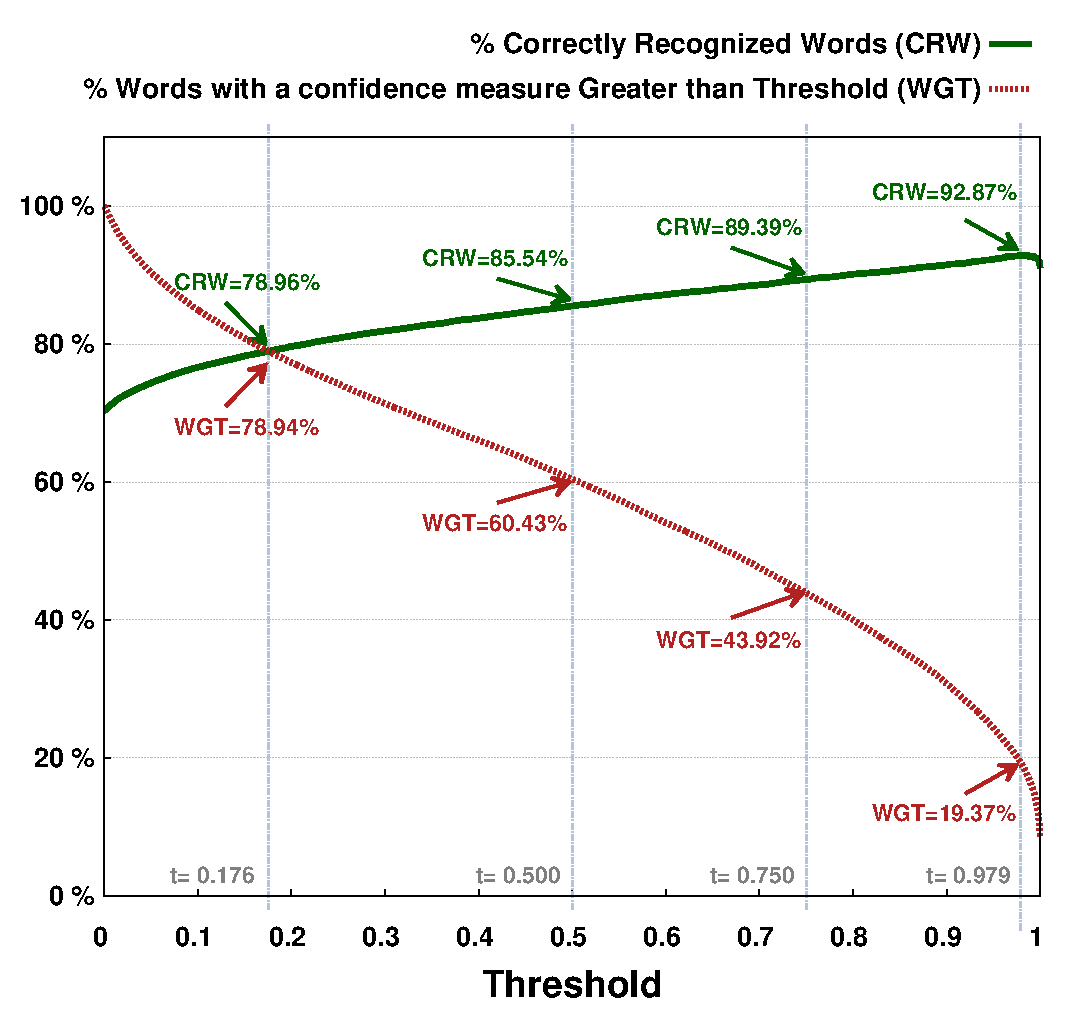
\includegraphics[scale=0.40]{Image/ETAPE_combined_min50occ_words}
               	\caption{results on word hypotheses}
        \end{subfigure}
	\hspace{0.3cm}
	\begin{subfigure}[b]{0.45\textwidth}
		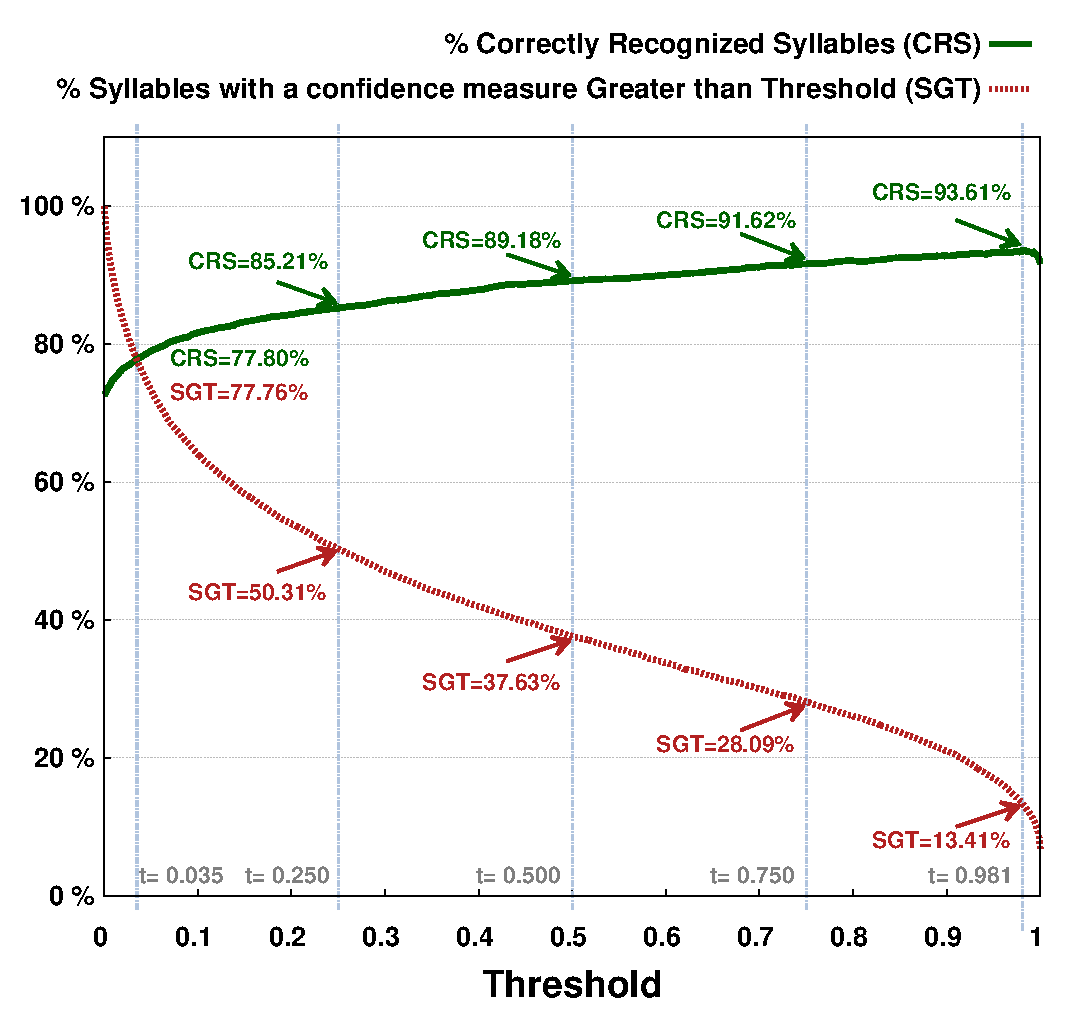
\includegraphics[scale=0.40]{Image/ETAPE_combined_min50occ_syllables}
                \caption{results on syllable hypotheses}
        \end{subfigure}
\caption{Analysis of the threshold's impact on the acceptance of words (a) and syllables (b) based on their confidence-measures: the red curves (WGT and SGT) indicate the percentage of units with a confidence measure greater than the threshold, and the green curves (CRW and CRS), the percentage of those correctly recognized. Evaluation on the ETAPE corpus, "min50occ" lexicon and language model}
\label{Fig:tc}
\end{figure*}


The results for the ETAPE corpus are displayed in Table \ref{Tab:RecWords}: the language model that combines the words seen at least 3 times with the syllables seen at least 3 times ("min3occ") generates 66K words (corresponding to 96.35\% of the units generated by the decoder), out of which 46K were correctly recognized (69.49\%). With the language model that combines the words seen at least 300 times with the syllables seen at least 3 times ("min300occ"), 70.29\% of words hypotheses are correctly recognized, but the number of recognized words is smaller (53K, corresponding to 61.99\% of units generated by the decoder). For ESTER2, the percentages of words generated by the decoder are similar to the values obtained for ETAPE. However, the percentages of correctly recognized words are somewhat higher (about 72\%).

Table \ref{Tab:RecWords} also shows the percentage of syllables that were correctly recognized. To obtain this percentage, two sequences of phonemes were compared: the sequence of phonemes corresponding to the recognized syllables (phonetic syllables) and the sequence of phonemes of the forced-aligned reference transcription (constrained by the syllable's time interval). If all the phonemes that compose a syllable are present in the reference, than that syllable is considered as correctly recognized. Keep in mind that there is also a significant amount of syllables that are only partially correct (considered as incorrect). The percentage of correctly recognized syllables varies between 56.06\% (for the "min3occ" language model, that outputs 2K syllables) and 77.55\% (for the "min300occ" language model, that outputs 33K syllables). For ESTER2, the percentages of correctly recognized syllables are about 3\% higher.

Another interesting approach is to filter the recognized words and the recognized syllables (obtained by the decoder) according to their confidence-measures, in order to maximize the percentage of units that are correct, i.e. correctly recognized by the system (CRW "correctly recognized words" and CRS "correctly recognized syllables").

The CRW ratio is calculated as follows:
	$$CRW(\sigma)=\frac{\text{\# words correctly recognized \& CM} \ge \sigma}{\text{\# words CM} \ge \sigma}$$

Figure \ref{Fig:tc} shows the performances achieved by setting up various thresholds between 0 and 1, when using the "min50occ" language model on the ETAPE corpus.

The figure \ref{Fig:tc}.(a) shows the threshold's impact on the acceptance of words. A threshold greater than 0.75 on the confidence measures leads to a CRW ratio greater than 89\%. However, a threshold too big rejects many words (for example, 80\% of the words have a confidence measure smaller than 0.97). The results obtained with the other language models and on the ESTER corpus are similar.

The figure \ref{Fig:tc}.(b) shows the threshold's impact on the acceptance of syllables. A threshold greater than 0.50 on the confidence measures leads to a CRS ratio greater than 89\%. However, a threshold too big rejects many syllables (for example, 86\% of the syllables have a confidence measure smaller than 0.98 and even 50\% of the syllables have a confidence measure smaller than 0.25). Regarding the results obtained with the other language models, the bigger the quantity of syllables in the language model, the better the results. For example, when using the "min3occ" language model (that models 0.11M syllables with 3.57M words), the contribution of the confidence measure on syllables is minimal : about 50\% of syllables have a confidence measure smaller than 0.07.

Increasing the threshold decreases the number of preserved linguistic units, but it increase the relevance of preserved hypotheses.
In practice a compromise must be made between the number of rejected linguistic units (considered as incorrect), and the performance that can be achieved on the preserved ones.



%%%%%%%%%%%%%%%%%%%%%%%%%%%%%%%%%%%%%%%%%%%%%%%%%%%%%%%%%%%%%%%%%%%%%%%%%%%%%%%%%%%%%%%%%%%%%%%%%%%%%%%%%%%%%%%%%%%%%%%%%%%
\section{Conclusions}

This paper analyzed the interest of using a hybrid language model of words and syllabes for speech transcription, as a support for helping communication with deaf people while implementing it on a portable terminal. This model aims to ensure proper recognition of the most frequent words and to offer suitable syllables for speech segments corresponding to out of vocabulary words.


The objective was to determine if combining words with syllables could still provide a good word recognition rate, and also to study the contribution and relevance of confidence measures to identify correctly recognized words.

The tests were carried out on two French speech corpora: ETAPE and ESTER2.
The percentage of words that are output by the recognizer varies between 96\% (when using the words seen at least 3 times during training) and 62\% (when using the words seen at least 300 times during training). Among the recognized words, about 70\% of them were correctly recognized.
By adjusting the threshold on the confidence measures of recognized words, we found, as expected, that the more we increase the threshold, the more we decrease the number of words having a confidence measure above it, and the more we will increase the ratio of correctly recognized words (between 70\% and 92\%). A compromise must be made between the number of words that are rejected, and the performance that can be obtained on the preserved words.
The contribution of confidence measures on syllables is relevant only if there is a fairly significant amount of syllables in the language model, as for example in the "min50occ" language model. The ratio of correctly recognized syllables varies then between 72\% and 94\%, while the amount of preserved syllables varies between 100\% and 13\%.

Future work will investigate further the confidence measures, in particular on short units, such as the syllables.

\section{Acknowledgements}
The work presented in this article is part of the RAPSODIE project, and has received
support from the “Conseil Régional de Lorraine” and from the “Région Lorraine” (FEDER) (http://erocca.com/rapsodie).

%\newpage
%
\eightpt
\bibliographystyle{IEEEtran/bibtex/IEEEtran}
\bibliography{myBib}
\end{document}
